\documentclass[11pt,oneside]{article}
\usepackage[T1]{fontenc}
\usepackage[utf8]{inputenc}
\usepackage{lmodern}
\usepackage[margin=1in]{geometry}
\usepackage{microtype}
\usepackage{amsmath,amssymb,amsthm,mathtools}
\usepackage{booktabs,longtable,tabularx,array,multirow}
\usepackage{enumitem}
\usepackage{xcolor}
\usepackage{listings}
\usepackage{fancyhdr}
\usepackage{hyperref}
\usepackage[nameinlink,noabbrev]{cleveref}
\usepackage{tikz}
\usetikzlibrary{arrows.meta,positioning,shapes.misc,fit,calc}
\usepackage{caption}
\usepackage{url}

\definecolor{linkblue}{RGB}{25,76,135}
\definecolor{codegray}{RGB}{247,247,247}
\definecolor{deepgreen}{RGB}{22,94,72}
\definecolor{warmred}{RGB}{148,54,43}
\hypersetup{
  colorlinks=true,
  linkcolor=linkblue,
  citecolor=linkblue,
  urlcolor=linkblue,
  pdftitle={Certified Bounded Interaction Programs for iPRA},
  pdfauthor={OpenAI research synthesis for the ProveIt project}
}
\setlist[itemize,enumerate]{leftmargin=*,topsep=0.3em,itemsep=0.18em}
\setlength{\parindent}{0pt}
\setlength{\parskip}{0.56em}
\setlength{\headheight}{14pt}
\setlength{\emergencystretch}{3em}
\setcounter{tocdepth}{2}
\setcounter{secnumdepth}{3}
\pagestyle{fancy}
\fancyhf{}
\fancyhead[L]{Certified Bounded Interaction Programs for iPRA}
\fancyhead[R]{\thepage}
\renewcommand{\headrulewidth}{0.4pt}

\lstset{
  basicstyle=\ttfamily\small,
  backgroundcolor=\color{codegray},
  frame=single,
  breaklines=true,
  columns=fullflexible,
  keepspaces=true,
  showstringspaces=false,
  keywordstyle=\bfseries\color{linkblue},
  commentstyle=\itshape\color{deepgreen},
  numbers=left,
  numberstyle=\tiny,
  xleftmargin=1.5em,
  framexleftmargin=1.2em
}

\newtheorem{theorem}{Theorem}[section]
\newtheorem{lemma}[theorem]{Lemma}
\newtheorem{proposition}[theorem]{Proposition}
\newtheorem{corollary}[theorem]{Corollary}
\newtheorem{definition}[theorem]{Definition}
\newtheorem{principle}[theorem]{Principle}
\newtheorem{barrier}[theorem]{Barrier}
\newtheorem{example}[theorem]{Example}
\theoremstyle{remark}
\newtheorem{remark}[theorem]{Remark}
\newtheorem{status}[theorem]{Status}

\newcommand{\iPRA}{\mathrm{iPRA}}
\newcommand{\PRA}{\mathrm{PRA}}
\newcommand{\Nat}{\mathbb{N}}
\newcommand{\Bool}{\mathbb{B}}
\newcommand{\Q}{\mathbb{Q}}
\newcommand{\Z}{\mathbb{Z}}
\newcommand{\CBIP}{\mathsf{CBIP}}
\newcommand{\Prf}{\mathsf{Prf}}
\newcommand{\PRAAx}{\mathsf{PRAAx}}
\newcommand{\PTm}{\mathsf{PTm}}
\newcommand{\Fm}{\mathsf{Fm}}
\newcommand{\Good}{\mathsf{Good}}
\newcommand{\Inv}{\mathsf{Inv}}
\newcommand{\Run}{\mathsf{Run}}
\newcommand{\Accept}{\mathsf{Accept}}
\newcommand{\Valid}{\mathsf{Valid}}
\newcommand{\Viable}{\mathsf{Viable}}
\newcommand{\Local}{\mathsf{Local}}
\newcommand{\Next}{\mathsf{Next}}
\newcommand{\Post}{\mathsf{Post}}
\newcommand{\Obs}{\mathsf{Obs}}
\newcommand{\Need}{\mathsf{Need}}
\newcommand{\CertCheck}{\mathsf{Check}}
\newcommand{\Val}{\mathsf{Val}}
\newcommand{\eqv}{\mathrel{\simeq}}
\newcommand{\code}[1]{\texttt{\detokenize{#1}}}

\title{\textbf{Certified Bounded Interaction Programs}\\[0.25em]
A General Proof-Producing Framework for Mathematics\\
in Intuitionistic Primitive Recursive Arithmetic}
\author{Research synthesis prepared for Vladimir Reshetnikov\\
and the ProveIt iPRA development}
\date{16 November 2026\\Repository snapshot: \texttt{210616e660a7ab5f0d706761c12bba673174cec9}}

\begin{document}
\maketitle

\begin{abstract}
The ProveIt repository now contains two sharply different layers: a kernel-checked object theory and a large collection of mathematically ambitious but mostly unverified proof packets.  Existing foundation packets already develop bounded Booleanization, finite traces, precision contracts, relational certificates, contract DAGs, and stable observers.  Their common remaining bottleneck is not another representation of computable mathematics, but a reusable route from local certificates to actual derivations of type \(\Prf\ \PRAAx\ \Gamma\ \varphi\).

This report develops \emph{Certified Bounded Interaction Programs} (CBIPs), a fixed-program intermediate language for finitary mathematical arguments.  CBIPs combine exact primitive-recursive transducers, queries to universally stated input contracts, bounded loops and searches, alternating finite challenges, relational producers, guarded partial operations, and quotient- or error-stable observers.  Every fixed CBIP normalizes to one bounded primitive-recursive trace with a quantifier-free invariant.  A small normalized reflection kernel then turns object-language base, step, and terminal derivations into the desired closed \(\Prf\ \PRAAx\) theorem.  The crucial compiler is metatheoretic and syntax directed: it generates explicit primitive-recursive symbols and proof terms for each fixed program, so it never assumes an impossible unclocked universal evaluator inside iPRA.

We give complete human proofs of bounded strategy determinacy with dual success/failure certificates, trace normalization, finite-use relational composition, stable witness erasure, adaptive finite use of global hypotheses, precision-DAG soundness, guarded arithmetic on represented objects, finite-net search, and height-bounded enumeration.  We also give explicit computability barriers showing why cardinality bounds do not yield search cutoffs, why horizonwise viability does not create a coherent infinite selector, why metastability does not yield a convergence rate, and why exact sign or branch selection is unavailable for arbitrary regular names.  The Lean plan is aligned with the current \code{PR}, \code{PTm}, \code{PRAAx}, \code{PRA.qfInd}, and checked \code{IPRADerivations} interfaces.  The archive includes a no-placeholder normalized trace-reflection candidate, detailed blueprints for the remaining compiler layers, and exact Python regression tests.  No completed Lean build or new kernel-checked theorem is claimed by this artifact.
\end{abstract}

\vspace{0.4em}
\noindent\textbf{Verification status.}
The report's mathematical arguments are intended to be complete at the stated level.  The Python reference algorithms were executed on exact integers and rational numbers.  The PDF was compiled, rendered, and inspected.  Lean is not installed in the artifact runtime and the repository cannot be cloned there; consequently, the Lean sources are source-oriented candidates and blueprints, not a claimed kernel check.  The status ledger separates proved-on-paper claims, executable finite evidence, checked upstream dependencies, and unfinished object-language work.

\tableofcontents
\newpage

\section{Scope, repository audit, and novelty boundary}

\subsection{The present repository situation}

The relevant ProveIt tree contains three logically distinct kinds of artifact.

\begin{enumerate}
\item \textbf{A checked foundation.}  \code{ConciseIPRA} defines ordinary first-order intuitionistic primitive recursive arithmetic by the types \code{PR}, \code{PTm}, the theory \code{PRAAx}, and the derivability relation \code{Prf PRAAx}.  Its checked bridges relate this ordinary presentation to the native scalar calculi.
\item \textbf{A checked derivation library.}  \code{IPRADerivations} contains explicit closed derivations
\[
   ([] : \mathsf{List}(\Fm\ \PTm\ 0))\;\vdash_{\PRAAx}\;\varphi
\]
for concrete arithmetic, algebraic, combinatorial, and number-theoretic statements.  Its reusable core already provides open induction, instantiation, equality congruence, semiring arithmetic, order, pairing, bounded sums and products, bounded search, division, gcd, finite matrices, and other infrastructure.
\item \textbf{Research packets.}  The packet collection contains broad human arguments, semantic Lean prototypes, numerical experiments, and formalization plans.  The repository explicitly distinguishes these from checked object-language derivations.  A report, a compiled host theorem, or a passing numerical test is therefore not automatically a theorem of iPRA.
\end{enumerate}

The close-out head was \texttt{210616e660a7ab5f0d706761c12bba673174cec9}.  Its latest commit added a fully object-level power-cleared Euler-product estimate, registered it in the checked derivation suite, and reported 432 checks with no \code{sorryAx}.  The core interfaces used by this report---\code{PR.lean}, \code{Deduction.lean}, \code{Core/Basic.lean}, and \code{Core/Search.lean}---were re-read at that head.  This is important methodologically: substantial finite inequalities are already being proved directly in the existing \code{Prf PRAAx} backend, so a new framework should reuse that backend rather than define a parallel logic.

\subsection{What the preceding frameworks already accomplish}

The foundation packets are unusually rich.  Collectively they already contain:

\begin{itemize}
\item bounded Booleanization and least bounded search;
\item deterministic trace reflection and certificate checking;
\item finite-observation semantics for represented objects;
\item precision-demand propagation and error-budget DAGs;
\item finite relational witnesses, backward viability, and finite-use composition;
\item stable or quotient-valued elimination of internal choices;
\item finite nets, explicit compact presentations, nested isolating regions, and metastability;
\item height-bound/complete-list conversion and careful separation of verifiers from difficult producers;
\item contract-DAG and proof-producing interface compiler architectures;
\item a source-level trace compiler outline whose remaining holes are precisely the de Bruijn and equality-transport steps needed to derive normalized base, successor, and terminal obligations.
\end{itemize}

It would be misleading to relabel those ideas and call them new.  The present contribution instead reorganizes them around the smallest missing trusted interface.

\subsection{The remaining common bottleneck}

Most packet-level proofs stop at one of the following boundaries.

\begin{enumerate}
\item A finite algorithm and invariant are described semantically, but no concrete \code{PR} symbol and no \code{Prf PRAAx} proof are produced.
\item A generic trace compiler is proposed, but it simultaneously handles program normalization, substitutions, recursion equations, and logical reflection.  The resulting theorem has a few difficult generic holes even though the final induction step is simple.
\item Bounded existential choices are handled, but arbitrary finite alternation---for example \(\forall q<Q\,\exists z<Z\,\forall e<E\)—is not integrated with relational and precision-aware computation.
\item A packet proves a finite verifier but does not identify whether the missing producer is routine engineering, an omitted quantitative hypothesis, or genuinely unavailable mathematics.
\end{enumerate}

The key design decision of this report is to split compilation into two layers.

\begin{definition}[Local normalization layer]
For a fixed program, the local layer elaborates each command into explicit primitive-recursive state updates and produces three derivations in the exact syntactic forms required by quantifier-free induction: a base derivation, a successor derivation, and a terminal extraction implication.
\end{definition}

\begin{definition}[Normalized reflection kernel]
The reflection kernel accepts only those already-normalized derivations.  It applies \code{PRA.qfInd}, specializes the resulting universal invariant at the computed fuel, applies terminal extraction, discharges the input guard, and universally closes the input variable.
\end{definition}

The second layer is tiny and independent of the mathematics.  All de Bruijn and equality rewriting is moved into local elaborators, where the relevant terms are visible and where the checked \code{IPRADerivations} lemmas can be used directly.  This split is both a mathematical normalization theorem and a practical Lean engineering strategy.

\subsection{Claim discipline}

We use four status labels throughout.

\begin{description}
\item[Human theorem.] A full mathematical argument is given, including finite bounds and the admissibility of each induction.
\item[Executable reference.] Exact finite code was run on representative instances.  This is regression evidence, not an iPRA proof.
\item[Object-level target.] A precise \code{Prf PRAAx} statement, dependencies, and proof-construction path are supplied.
\item[Checked upstream result.] The statement is already in the repository's checked libraries at the audited snapshot.  This package does not independently rebuild the repository.
\end{description}

No generic theorem in this report is to be read as creating a difficult mathematical producer.  A finite checker can validate a height certificate, a zero-free region, a root-count table, or a modulus.  It cannot manufacture such data merely because the downstream verification is finite.

\subsection{Road map}

\Cref{sec:interfaces} describes mathematical concepts by finitary interfaces.  \Cref{sec:cbip} defines the bounded interaction language.  \Cref{sec:games} handles arbitrary fixed bounded alternation.  \Cref{sec:compiler} proves trace normalization and reflection.  \Cref{sec:relational} adds finite relational evidence and stable witness erasure.  \Cref{sec:quantitative} develops represented arithmetic and precision contracts.  Later sections give domain patterns, impossibility boundaries, a difficulty-resolution matrix, and a Lean implementation plan.

\section{Mathematical concepts as finitary interfaces}\label{sec:interfaces}

\subsection{Why an interface is more useful than a completed infinite object}

An ordinary mathematical proof may speak about a real number, a continuous function, a compact space, a multiset of algebraic roots, a probability distribution, or a finitely generated group.  None of these need be inserted into iPRA as a completed set-theoretic object.  What a finite proof actually uses is a finite collection of observations: rational approximations, coefficient values, residual inequalities, chart membership, finite sums, or answers to bounded searches.

This motivates a uniform observation interface.

\begin{definition}[Finitary presentation]
A finitary presentation \(\mathcal A\) consists of fixed primitive-recursive data
\[
  \mathsf{Par}_{\mathcal A},\qquad
  B_{\mathcal A}(p,q),\qquad
  \Valid_{\mathcal A}(p,q,a),\qquad
  \mathsf{Compat}_{\mathcal A}(p,q,a,q',a'),
\]
where \(p\) is a parameter code, \(q\) is a finite query, and \(a<B_{\mathcal A}(p,q)\) is a bounded answer.  All predicates are numerical Booleans.  Optionally the presentation supplies:
\begin{itemize}
\item an observational equivalence \(E_{\mathcal A}(p,q,a,a')\);
\item a coded distance or diameter bound;
\item a refinement relation between levels;
\item a producer certificate showing that a valid answer exists for the queried level.
\end{itemize}
\end{definition}

The bound may be enormous; only primitive recursiveness and explicitness matter.  A presentation can be deterministic by having exactly one valid answer, relational by allowing several, or adversarial by exposing all bounded challenges that a proof must survive.

\subsection{Examples of the interface}

\paragraph{Exact finite algebra.}
An integer polynomial is a finite coefficient code.  A query asks for a coefficient, degree, product coefficient, resultant entry, or evaluation at a coded integer.  Validity is exact equality.  No approximation or relational choice is needed.

\paragraph{Regular real names.}
The parameter \(p\) codes a fixed evaluator \(a(p,n)\in\Q\).  A query is a precision index \(n\), and the answer is the uniquely encoded rational sample.  A global regularity contract supplies the finite inequalities used to compare requested samples.  Extensional equality is itself an all-precision observation, but any particular theorem uses only finitely many instances before universally introducing its requested output precision.

\paragraph{Root clusters.}
A query is a requested diameter.  An answer is a finite list of rational boxes or disks with multiplicities and root-count certificates.  Several refinements may be valid.  Compatibility asserts that a finer clustering refines the coarser one.  Symmetric polynomials or factor products are stable observations even when individual labels are not.

\paragraph{Projective and geometric data.}
A projective point is represented by a nonzero vector modulo scaling, not by a globally normalized vector.  Queries ask for a chart, determinant, incidence test, or bounded-precision coordinate ratio.  Several overlapping charts may be valid.  Exact normalization is guarded by an explicit pivot or norm lower bound.

\paragraph{Effective compact domains.}
A query \(k\) asks for a finite \(2^{-k}\)-net and a coverage certificate.  The answer is a finite point list plus finite witnesses for the relevant cells.  Compactness is not an axiom; it is a family of finite presentations whose coverage theorem is a producer obligation.

\paragraph{Diophantine solution sets.}
Given a height bound \(H(p)\), the answer to the sole query is the boundedly filtered list of all codes below \(H(p)\) satisfying the equation.  The verifier and enumerator are generic.  The difficult mathematical content is the producer proving that every solution has height at most \(H(p)\).

\subsection{Observation and realization}

A theorem about a presented object should be stated at the level actually observed.  A deterministic observation has the form
\[
  \forall p\,\forall k\; \Good(p,k)=1\;\longrightarrow\;
  \Obs(p,k,F(p,k))=1,
\]
where \(F\) is a fixed primitive-recursive evaluator.  A relational observation has the form
\[
  \forall p,k,c\; \CertCheck(p,k,c)=1\;\longrightarrow\;
  \Obs(p,k,\mathsf{out}(c))=1.
\]
A quotient-valued observation replaces literal equality of outputs by a decidable relation \(E\).  An approximate observation replaces equality by a rational diameter bound.

This formulation has three advantages.

\begin{enumerate}
\item It never requires the object theory to quantify over functions or completed infinite objects.
\item It exposes exactly which samples, bounds, and certificates are consumed.
\item It makes nonuniqueness harmless when the conclusion is invariant or stable under the allowed relation.
\end{enumerate}

\subsection{Finite use of global contracts}

Suppose a name or structure is supplied by a global formula
\[
  \mathsf{Reg}(p)\;\equiv\;\forall m\,\forall n\;R(p,m,n,a(p,m),a(p,n)).
\]
A bounded computation may choose its next query adaptively from earlier answers.  The correct invariant does not include the whole universal formula.  It contains a finite table of the instances already used.  At a successor step, the proof uses universal elimination at the computed terms, inserts the resulting Boolean fact into the table, and continues.

\begin{lemma}[Adaptive finite instantiation]
For every fixed bounded computation making at most \(N(u)\) adaptive queries to a universally quantified primitive-recursive contract, there is a primitive-recursive table update and a quantifier-free invariant saying that every stored contract instance is valid.  iPRA proves preservation of this invariant by quantifier-free induction.
\end{lemma}

\begin{proof}
Encode the finite list of queries and answers in the state.  At step \(i\), the next query \(q_i\) is a term in the current state.  Universal elimination of the external contract at \(q_i\), and at any previously stored index with which it must be compared, produces the new finite facts.  A bounded Boolean fold verifies old entries and the new row.  The invariant is one equation asserting that this fold equals one.  Its base case is the empty table; its successor case follows from the instantiated contract and the defining equation of the table update.  No universal quantifier occurs in the induction formula.
\end{proof}

\subsection{Interface composition}

Let \(F:\mathcal A\to\mathcal B\) and \(G:\mathcal B\to\mathcal C\) be finite interfaces.  A query to \(G\) induces finitely many queries to the output of \(F\); these in turn induce finitely many queries to the original input.  The composed demand is found by a backward pass, while the actual answers are generated by a forward trace.

If all interfaces are deterministic, composition is ordinary substitution of primitive-recursive programs.  If an intermediate interface is relational, composition is valid only relative to the finite consumer's actual interaction tree.  That case is developed in \Cref{sec:relational}.  If an intermediate operation is partial, its interface contains a Boolean guard and the composition proof must show that the preceding component supplies the guard.  This prevents totalized default branches from being used as though they were mathematically valid.

\section{Certified Bounded Interaction Programs}\label{sec:cbip}

\subsection{The fixed-program principle}

A primitive-recursive language may contain one symbol for every fixed program built from zero, successor, projections, composition, and primitive recursion.  It must not contain an unclocked evaluator for arbitrary codes of all primitive-recursive programs: such an evaluator would diagonalize outside the primitive-recursive class.  Accordingly, a CBIP is compiled externally, one fixed syntax tree at a time.  The compiler produces explicit \code{PR} syntax and explicit proof terms; the object theory reasons only about the resulting fixed symbols.

\begin{principle}[No internal universal evaluator]
Every theorem in the framework is a schema indexed by a fixed CBIP.  Structural recursion on the program is metatheoretic code generation.  Object-theoretic recursion is used only for the finitely many loops occurring in the compiled program.
\end{principle}

\subsection{Program constructors}

A CBIP state is a bounded numerical code containing a program counter, user parameters, finite stores, certificates, and error metadata.  The core constructors are as follows.

\begin{description}
\item[Exact update \(\mathsf{emit}(f)\).] Replace a store component by a fixed primitive-recursive term \(f\).
\item[Assertion \(\mathsf{assert}(r)\).] Check a Boolean relation.  A failed assertion moves to a designated rejecting state; soundness uses only the accepting branch.
\item[Global-contract query \(\mathsf{query}(H,q)\).] Instantiate an external universally quantified hypothesis at the computed query \(q\) and store the resulting finite fact.
\item[Bounded loop \(\mathsf{loop}(b,P)\).] Execute \(P\) at most \(b(u)\) times.  The local invariant must be quantifier free after Booleanization.
\item[Least bounded search \(\mathsf{search}(b,r)\).] Return the least \(i<b\) satisfying \(r(i)=1\), or the sentinel \(b\).
\item[Existential choice \(\mathsf{pick}(b,r)\).] Consume a certificate for one valid answer below \(b\).  It may be implemented by search when validity is decidable and existence is proved.
\item[Universal challenge \(\mathsf{challenge}(b,P)\).] Verify the continuation for every \(i<b\), or consume an all-children strategy certificate.
\item[Relational query \(\mathsf{rel}(b,\Local,\Next)\).] Permit any locally valid answer whose successor state remains viable for the remaining finite horizon.
\item[Guarded operation \(\mathsf{guard}(g,P,Q)\).] Branch on a decidable numerical guard.  Mathematical uses of a totalized partial operation must prove the intended guard.
\item[Stable observation \(\mathsf{observe}(E,o)\).] Export an output only modulo a supplied equivalence \(E\), or within a supplied diameter.  This erases internal finite choices when the final theorem does not depend on them.
\item[Sequential and finite parallel composition.] Combine programs by a phase tag or by a product state.  Parallel computations remain finite and can be scheduled sequentially.
\end{description}

The language is deliberately first order.  Higher-type-looking behavior, such as querying a real name or a modulus, is compiled into calls to fixed numerical evaluators and finite instances of their contracts.

\subsection{Typing by resources and observations}

A useful implementation assigns each wire an interface type and each command an effect.

\begin{center}
\begin{tabularx}{\textwidth}{@{}lXl@{}}
\toprule
Type/effect & Meaning & Typical evidence \\
\midrule
\code{Exact C} & exact finite code & defining equations \\
\code{Name C} & precision-indexed samples & regularity/modulus \\
\code{Rel C} & finite family of admissible answers & local validity and viability \\
\code{Guard G C} & operation valid under guard \(G\) & apartness, positivity, isolation \\
\code{Quot E C} & output used modulo \(E\) & confluence/invariance \\
\code{Approx d C} & outputs have certified diameter \(d\) & stability/Lipschitz bound \\
\code{Cert P} & externally generated finite certificate & checker soundness \\
\bottomrule
\end{tabularx}
\end{center}

Typing prevents several common mistakes.  A \code{Name} cannot be divided without a \code{Guard}; a \code{Rel} cannot silently become \code{Exact}; a metastable window is not a tail modulus; and a \code{Cert} proves only what its checker soundness theorem states.

\subsection{Operational semantics}

For a fixed input \(u\), the normalized machine has primitive-recursive functions
\[
  \Good(u),\quad \mathsf{init}(u),\quad \mathsf{fuel}(u),\quad
  \mathsf{step}(i,s,u),\quad \Inv(i,s,u),\quad \Accept(s,u).
\]
The run is
\[
  \Run(0,u)=\mathsf{init}(u),\qquad
  \Run(i+1,u)=\mathsf{step}(i,\Run(i,u),u).
\]
The compiler uses a total step function.  Finished and rejected states are frozen.  Thus the fixed fuel need not equal the exact stopping time.  The invariant records a status tag and proves that an accepting terminal state satisfies the desired observation.

\subsection{One trace, not one loop per mathematical paragraph}

Nested loops, finite searches, certificate checks, and local computations can all be flattened into one outer trace.  The state contains the program counter and each live local counter.  A lexicographic schedule or a precomputed static bound gives a single fuel.  This normalization is valuable for iPRA because it concentrates induction into one quantifier-free invariant.

The state may grow, but proof size is not forced to grow in the same way.  Local equations and certificate-checker lemmas are proved separately and invoked in the global successor case.  In Lean, this means the global trace theorem is a short composition of checked local derivations rather than an enormous arithmetic proof reconstructed from first principles.

\subsection{Proof-producing versus proof-carrying execution}

Two modes coexist.

\begin{enumerate}
\item In \emph{recomputation mode}, the object theory runs the primitive-recursive program and proves its invariant.
\item In \emph{certificate mode}, an external tool supplies a finite trace, viability table, interval subdivision, or strategy tree.  A smaller primitive-recursive checker validates it, and an object theorem reflects acceptance into the desired conclusion.
\end{enumerate}

Certificate mode does not weaken trust: the external producer is untrusted.  It often reduces proof-term size and permits sophisticated search to occur outside the kernel.  The trusted content is the fixed checker and its \code{Prf PRAAx} soundness derivation.

\section{Bounded formulas as finite strategy games}\label{sec:games}

\subsection{Booleanization with proof-relevant output}

A bounded formula is built from primitive-recursive decidable atoms by propositional connectives and quantifiers
\[
  \exists i<b(\vec x,\vec z)\,A(\vec x,\vec z,i),\qquad
  \forall i<b(\vec x,\vec z)\,A(\vec x,\vec z,i),
\]
where the bound may depend on earlier variables but not on \(i\).  Ordinary Booleanization returns only a truth value.  For proof engineering, it is more useful to return a strategy certificate explaining either success or failure.

Define Boolean folds
\[
 \mathsf{any}(b,f)=\max_{i<b} f(i),\qquad
 \mathsf{all}(b,f)=\prod_{i<b} f(i),
\]
with empty values zero and one, respectively.  Define \(\mathsf{first}(b,f)\) as the least successful index, or the sentinel \(b\) if none exists.  All three are fixed primitive recursions.

\begin{lemma}[Least-success invariant]\label{lem:first}
For every Boolean-valued primitive-recursive predicate \(f\), iPRA proves
\begin{align*}
  \mathsf{first}(b,f)&\leq b,\\
  \mathsf{first}(b,f)<b&\longrightarrow f(\mathsf{first}(b,f))=1,\\
  j<\mathsf{first}(b,f)&\longrightarrow f(j)=0.
\end{align*}
If \(\mathsf{first}(b,f)=b\), then every \(j<b\) fails.
\end{lemma}

\begin{proof}
Maintain a register \(s_i\leq i\).  Initially \(s_0=0\).  At stage \(i\), if \(s_i<i\), retain the previously found witness.  Otherwise \(s_i=i\), so no earlier index succeeded; set \(s_{i+1}=i\) when \(f(i)=1\), and \(s_{i+1}=i+1\) otherwise.  The invariant says that \(s_i<i\) exactly when a success occurs below \(i\), and in that case \(s_i\) is the least one.  Bounded statements about earlier indices are represented by Boolean folds, so the induction formula is quantifier free.  At \(i=b\) the displayed consequences follow.  The checked \code{IPRADerivations.Core.Search} module already contains a closely related least-zero search and its minimality theorem, so a Lean implementation should adapt that code rather than introduce a second search library.
\end{proof}

\subsection{The game associated with a bounded formula}

Push negations to atoms, which is intuitionistically valid because every atom is decidable.  Interpret conjunction and bounded universal quantification as moves by an adversary; interpret disjunction and bounded existential quantification as moves by a prover.  A leaf is won by the prover exactly when its Boolean atom is one.  The resulting tree is finite for every numerical input, although its branching bound may depend on earlier moves.

A success certificate stores one winning child at prover-controlled nodes and certificates for every child at adversary-controlled nodes.  A failure certificate does the dual: one losing child at adversary-controlled nodes and failure certificates for every child at prover-controlled nodes.  Thus failure is not an opaque zero; it carries a bounded counterstrategy.

\begin{theorem}[Two-sided bounded strategy compilation]\label{thm:strategy}
For every fixed bounded formula \(A(\vec x)\), one can primitive-recursively construct:
\[
  \Val_A(\vec x)\in\{0,1\},\qquad
  \mathsf{cert}_A(\vec x),\qquad
  \CertCheck_A(\vec x,w,c)\in\{0,1\},
\]
such that iPRA proves
\begin{align*}
 \Val_A(\vec x)=1 &\leftrightarrow A(\vec x),\\
 \CertCheck_A(\vec x,\Val_A(\vec x),\mathsf{cert}_A(\vec x))&=1,\\
 \CertCheck_A(\vec x,1,c)=1&\longrightarrow A(\vec x),\\
 \CertCheck_A(\vec x,0,c)=1&\longrightarrow \neg A(\vec x).
\end{align*}
The checker is a bounded primitive-recursive program, and every internal induction is quantifier free after replacing bounded quantifiers by folds.
\end{theorem}

\begin{proof}
Proceed by structural recursion on the fixed formula in the metatheory.

For an atom, compute its Boolean value.  The certificate records that value, and the checker recomputes it.  Soundness is the atom's decidability theorem.

For \(B\vee C\), the prover wins when one child has value one.  In the winning case, store the least winning side and its success certificate.  In the losing case, store failure certificates for both children.  The checker verifies the tag and the relevant subcertificates.  Conjunction is dual.

For \(\exists i<b\,B(i)\), compute the bounded \(\mathsf{any}\) fold.  If it is one, \Cref{lem:first} returns the least winning \(i<b\), and the certificate stores \(i\) and a success certificate for \(B(i)\).  If it is zero, the certificate stores a bounded table of failure certificates for every \(i<b\).  The checker iterates through the table; the fold invariant proves every instance false.  For \(\forall i<b\,B(i)\), interchange success and failure roles: success contains all child certificates, while failure contains one least counterexample.

The formula depth is fixed at compile time.  Structural recursion therefore generates a finite nest of concrete primitive recursions; it is not an object-language recursion over arbitrary formula codes.  Correctness of each bounded fold is proved by quantifier-free induction.  Composing those derivations yields the four displayed formulas.
\end{proof}

\subsection{Failure-producing contracts}

Many mathematical interfaces naturally have the shape
\[
 C(a)\equiv \forall q<Q(a)\;\exists z<Z(a,q)\;\forall e<E(a,q,z)\;R(a,q,z,e).
\]
Here \(q\) is a demanded precision or challenge, \(z\) is a proposed finite witness, and \(e\) ranges over local verifier tests.  Applying \Cref{thm:strategy} gives more information than a Boolean decision.

\begin{corollary}[Finite challenge decomposition]
There are primitive-recursive constructors and checkers producing exactly one of the following finite certificates.
\begin{enumerate}
\item A strategy assigning each \(q<Q(a)\) a witness \(z(a,q)<Z(a,q)\) that passes every local test \(e<E(a,q,z(a,q))\).
\item A counterchallenge \(q_0<Q(a)\) and, for every candidate \(z<Z(a,q_0)\), a failing test \(e_0(z)<E(a,q_0,z)\).
\end{enumerate}
The corresponding soundness alternatives are provable in iPRA.
\end{corollary}

This interface is useful even when the positive producer is not known.  It gives a reproducible finite obstruction, prevents arbitrary choice from being mistaken for an existential witness, and localizes which demanded precision or certificate field failed.

\subsection{Classical reasoning on bounded conclusions}

Bounded formulas are decidable because they have Boolean realizers.  Hence iPRA proves \(A\vee\neg A\) and \(\neg\neg A\to A\) for every fixed bounded \(A\).  Consequently, a classical finite argument can often be imported as follows: apply a negative translation to obtain \(\neg\neg A\), then eliminate the double negation using the compiled decidability of \(A\).  This does not transfer arbitrary unbounded classical conclusions.  The elimination is valid precisely because the retained endpoint is a finite Boolean observation.

\section{Normalization to one trace and object-level reflection}\label{sec:compiler}

\subsection{Deterministic trace reflection}

A normalized trace system consists of fixed primitive-recursive symbols
\[
  \Good(u),\quad \mathsf{init}(u),\quad \mathsf{fuel}(u),\quad
  \mathsf{step}(i,s,u),\quad \Inv(i,s,u),\quad \Accept(s,u).
\]
Define \(\Run\) by primitive recursion on \(i\).  The local obligations are
\begin{align}
 \Good(u)=1 &\longrightarrow \Inv(0,\mathsf{init}(u),u)=1, \tag{B}\label{eq:base}\\
 \Good(u)=1\wedge \Inv(i,s,u)=1
   &\longrightarrow \Inv(i+1,\mathsf{step}(i,s,u),u)=1, \tag{S}\label{eq:step}\\
 \Good(u)=1\wedge \Inv(\mathsf{fuel}(u),s,u)=1
   &\longrightarrow \Accept(s,u)=1. \tag{F}\label{eq:finish}
\end{align}
All are quantifier-free formulas after Booleanization.

\begin{theorem}[Normalized trace reflection]\label{thm:trace-reflection}
If the object theory contains derivations of the normalized base, successor, and terminal obligations, then it contains a derivation
\[
  \vdash_{\PRAAx}\forall u\,
  \bigl(\Good(u)=1\to
    \Accept(\Run(\mathsf{fuel}(u),u),u)=1\bigr).
\]
\end{theorem}

\begin{proof}
Keep \(u\) free.  Use the quantifier-free induction formula
\[
 I(i,u)\equiv \Inv(i,\Run(i,u),u)=1.
\]
The normalized base derivation proves \(I(0,u)\) under \(\Good(u)=1\).  The normalized successor derivation already includes the rewrite
\[
 \Run(i+1,u)=\mathsf{step}(i,\Run(i,u),u),
\]
so it proves \(I(i+1,u)\) from \(I(i,u)\) in the shifted context.  Apply \code{PRA.qfInd} to obtain \(\forall i\,I(i,u)\), then apply \code{Prf.allE} at \(\mathsf{fuel}(u)\).  The terminal implication gives acceptance.  Finally apply implication introduction to discharge \(\Good(u)=1\) and universal introduction to close \(u\).
\end{proof}

The proof is intentionally smaller than earlier raw-contract compilers.  Run-zero, run-successor, and equality transport are not hidden inside this kernel.  They belong to the local normalization layer, where theorem-specific terms can be rewritten by the checked \code{PRA.precZero}, \code{PRA.precSucc}, \code{Prf.eqCongr}, and \code{Prf.eqSubst1} lemmas.  The accompanying \code{NormalizedTraceReflection.lean} is a source-level candidate for this exact theorem and contains no placeholder proof.

\subsection{The CBIP normalization theorem}

\begin{theorem}[Fixed-program normalization]\label{thm:normalization}
For every fixed CBIP \(P\) whose loops and bounded interactions have primitive-recursive bounds, one can construct a normalized trace system \(T_P\) such that:
\begin{enumerate}
\item the run of \(T_P\) simulates the operational semantics of \(P\);
\item \(\Inv_P\) is quantifier free;
\item the fuel \(F_P(u)\) is primitive recursive;
\item every accepting terminal state yields the declared observation of \(P\);
\item from object-language local contracts for the primitive commands, the compiler constructs normalized base, successor, and terminal derivations for \(T_P\).
\end{enumerate}
Therefore \Cref{thm:trace-reflection} produces the closed object-iPRA theorem for \(P\).
\end{theorem}

\begin{proof}
The construction is by structural recursion on the fixed syntax of \(P\).  The state contains a program counter, all live variables, finite tables, loop counters, and a status tag.  The invariant is a Boolean case split on the program counter.  We describe each constructor.

\emph{Exact update.}  The step replaces the designated register by the fixed term.  The invariant's next clause follows from the defining equation of that term and congruence.

\emph{Assertion and guard.}  The numerical Boolean is decidable.  The step enters the success or failure tag.  In the success branch, the checked equality is stored in the invariant; in the failure branch, the state is frozen.  The global theorem is conditional on reaching acceptance, so no false mathematical conclusion is extracted from the rejected branch.

\emph{Sequential composition.}  Add a phase tag.  In the first phase use the first component invariant.  At the switch, store its terminal certificate and initialize the second component.  In the second phase use the second invariant together with the frozen first certificate.  The fuel is the sum of the component fuels plus one switch step.

\emph{Finite parallel composition.}  Schedule the components sequentially in a product state.  The invariant is the conjunction of completed component certificates and the current component invariant.  Since the number of components is fixed or primitively bounded by input data, this is a bounded loop.

\emph{Bounded loop.}  Store the outer counter and the inner local state.  The compiler either assigns a static block of fuel to each iteration or flattens the pair of counters lexicographically.  The invariant says that all completed iterations satisfy their postconditions and that the active iteration satisfies its local invariant.  A finite fold replaces the phrase ``all completed iterations.''

\emph{Least bounded search.}  Use the checked least-search recurrence or an equivalent sentinel register.  Its invariant is \Cref{lem:first}.  The terminal state contains either a least witness or a proof that every candidate failed.

\emph{Global-contract query.}  The next query is a term in the current state.  Universal elimination instantiates the external hypothesis at that term.  A bounded table update stores the resulting Boolean fact, preserving the finite-query invariant.

\emph{Existential and universal challenge.}  Compile the fixed bounded subformula by \Cref{thm:strategy}.  Certificate verification is itself a deterministic bounded trace.  The invariant records the checked prefix of the strategy tree.

\emph{Relational query.}  First run a backward viability-table trace, then a forward least-viable replay trace.  The switch certificate states that the initial state is viable.  Detailed correctness appears in \Cref{sec:relational}.

\emph{Stable observation.}  The terminal extraction proof combines the generated certificate with a supplied confluence, quotient-invariance, or diameter estimate.  Internal witnesses do not appear in the closed conclusion.

Every constructor introduces only fixed primitive-recursive terms, bounded folds, or primitive recursion.  Every invariant clause is an equation or Boolean combination of equations.  The proof compiler composes local \code{Prf PRAAx} derivations using substitution, weakening, implication elimination/introduction, equality transport, and finite case splits.  This yields the three normalized derivations required by \Cref{thm:trace-reflection}.
\end{proof}

\subsection{Why the compiler theorem is a schema}

The normalization proof does not assert that iPRA itself evaluates arbitrary program syntax.  A Lean metaprogram or ordinary definition traverses the fixed CBIP and emits:
\begin{itemize}
\item one concrete \code{PR} runner;
\item one concrete quantifier-free formula;
\item concrete local proof terms assembled from a finite library.
\end{itemize}
The emitted theorem is then checked by Lean's kernel.  This is analogous to a verified macro expansion: correctness is expressed by the generated object proof, not by trusting the generator.

\subsection{Contract DAGs and reverse demand propagation}

For a finite acyclic computation graph, each node advertises its local input demands and output contract.  Given a requested output precision \(k\), a reverse topological pass computes every predecessor demand.  A forward trace then evaluates nodes in topological order.  The global invariant says:
\begin{enumerate}
\item all processed nodes satisfy their local contracts;
\item the stored demand table equals the reverse recurrence;
\item every guard and magnitude bound required downstream has been established;
\item the accumulated error budget is below the assigned node budget.
\end{enumerate}
The reverse pass and forward pass may be two traces combined by the compiled stable-observer glue, or one trace with a phase tag.  This subsumes prior contract-DAG proposals while making their final reflection step explicit.

\subsection{Certificate reflection}

An external producer may supply the entire trace \(c=(s_0,\dots,s_N)\).  A checker verifies the initial state, every transition, every invariant row, and terminal acceptance.  A separate bounded induction proves \(s_i=\Run(i,u)\).  Hence
\[
  \CertCheck_{\mathrm{trace}}(u,c)=1\longrightarrow
  \Accept(\mathsf{last}(c),u)=1.
\]
The certificate may omit redundant states if it contains a DAG with replay pointers; the checker then follows a decreasing resource or topological index.  This permits large searches to be performed externally while retaining a small trusted arithmetic core.

\section{Finite relational evidence and stable witness erasure}\label{sec:relational}

\subsection{Bounded evidence machines}

A relational producer need not return one globally coherent object.  For a finite consumer, it is enough to expose finitely many locally valid responses.  Fix an input \(x\), a remaining resource \(r\), and a consumer state \(s\).  A bounded evidence machine has primitive-recursive fields
\[
 \mathsf{halt}(x,r,s),\quad \Post(x,r,s),\quad
 A(x,r,s),\quad \Local(x,r,s,a),\quad \Next(x,r,s,a).
\]
If the state is terminal, \(\Post\) is the desired finite conclusion.  Otherwise an answer \(a<A(x,r,s)\) is admissible when \(\Local=1\), and the consumer continues at \(\Next\) with one less unit of resource.  The state stores all history needed for compatibility.

\subsection{Backward viability}

Define the Boolean \(\Viable(x,r,s)\) by primitive recursion on \(r\).  To keep the recurrence readable, put
\begin{align*}
 T(x,r,s)&:=\mathsf{halt}(x,r,s)\cdot\Post(x,r,s),\\
 D(x,r+1,s)&:=\max_{a<A(x,r+1,s)}\!\Bigl(
   \Local(x,r+1,s,a)\cdot
   \Viable(x,r,\Next(x,r+1,s,a))\Bigr),\\
 C(x,r+1,s)&:=(1-\mathsf{halt}(x,r+1,s))\cdot D(x,r+1,s).
\end{align*}
Then
\[
 \Viable(x,0,s)=T(x,0,s),\qquad
 \Viable(x,r+1,s)=\max\bigl(T(x,r+1,s),C(x,r+1,s)\bigr).
\]
Every maximum is a bounded Boolean fold.

\begin{theorem}[Finite viability correctness]\label{thm:viability}
For every fixed evidence machine, iPRA proves that \(\Viable(x,r,s)=1\) exactly when there is a successful transcript of length at most \(r\) from \(s\).  The transcript predicate is bounded and can itself be Booleanized.
\end{theorem}

\begin{proof}
Induct on \(r\).  At zero, success means immediate termination with the postcondition, which is the defining equation.  At \(r+1\), split on the numerical halt Boolean.  In the terminal branch, viability is exactly \(\Post\).  In the nonterminal branch, success consists of an answer below the finite bound satisfying \(\Local\) and a successful continuation at resource \(r\).  Apply the induction hypothesis to the continuation and the bounded-existential fold theorem to the answer.  The induction predicate is an equality of numerical Booleans, hence quantifier free.
\end{proof}

\subsection{Least viable execution}

At a nonterminal viable state, choose the least answer satisfying
\[
 \Local(x,r,s,a)=1\quad\text{and}\quad
 \Viable(x,r-1,\Next(x,r,s,a))=1.
\]
The least-success theorem gives such an answer.  Define forward execution by primitive recursion, appending the selected answer and decrementing the resource.

\begin{theorem}[Finite-use relational composition]\label{thm:rel-compose}
If \(\Viable(x,h,\mathsf{start}(x))=1\), the least-viable execution returns within \(h\) answer steps a transcript whose edges satisfy \(\Local\) and whose terminal state satisfies \(\Post\).  The theorem is provable in iPRA by quantifier-free induction.
\end{theorem}

\begin{proof}
The invariant at executed-step count \(i\) says:
\begin{enumerate}
\item the stored transcript has length \(i\);
\item replaying \(\Next\) along it gives the current state;
\item every stored edge satisfies \(\Local\);
\item the current state is viable for the remaining resource \(h-i\).
\end{enumerate}
All list and bounded-universal claims are Boolean folds.  The base is the empty transcript and the assumed initial viability.  At a nonterminal state, unfold the viability equation.  Its existential fold is one, so least search returns a locally valid answer with viable successor.  Append it and preserve the invariant.  The resource strictly decreases, so after at most \(h\) answer steps either a terminal state has been reached or the zero-resource viability equation forces one.  The terminal invariant yields \(\Post=1\).
\end{proof}

This theorem composes a multivalued producer with one bounded adaptive consumer.  It does not choose an infinite branch and does not assert that executions selected for different horizons agree.

\subsection{Strategy and relational choice are one mechanism}

The game compiler of \Cref{sec:games} is a special case of backward viability.  At a prover node, locally valid answers are candidate moves; at an adversary node, the certificate state requires all children to be checked.  Conversely, relational viability may be viewed as a game in which the producer proposes a local answer and the checker challenges compatibility and terminal postconditions.  A unified Lean library can therefore share Boolean folds, state encodings, certificate tables, and replay lemmas.

\subsection{Exact branch-invariant elimination}

Let \(o(t)\) be the output of a successful terminal transcript and let \(E(x,y,z)\) be a primitive-recursive equivalence relation appropriate to the theorem: literal equality, permutation equivalence, projective equivalence, equality of a symmetric polynomial, or equality of encoded finite sets.

\begin{theorem}[Stable quotient output]\label{thm:stable-quotient}
Assume initial viability and an object-iPRA proof that any two successful terminal states reachable within the finite horizon have \(E\)-equivalent outputs.  Then the output of the least-viable execution is \(E\)-equivalent to every successful output.  If \(E\) is equality, the chosen code is unique; otherwise the theorem exports the quotient-level observation without exposing the internal branch.
\end{theorem}

\begin{proof}
By \Cref{thm:rel-compose}, the selected execution is successful.  Instantiate the finite confluence theorem with the selected terminal state and an arbitrary successful one.  The resulting \(E\)-proof is exactly the desired conclusion.  No compatibility between choices at different horizons is required.
\end{proof}

\subsection{Quantitative witness erasure}

Exact confluence is often stronger than needed.  Suppose a coded metric \(d\) and rational \(\delta\) satisfy
\[
 \mathsf{Success}(t_1)\wedge \mathsf{Success}(t_2)
 \longrightarrow d(o(t_1),o(t_2))\leq\delta.
\]
Then the selected output is within \(\delta\) of every admissible output.  If a downstream observer is \(L\)-Lipschitz, its values differ by at most \(L\delta\).  At requested precision \(k\), choose the relational level so that this final diameter fits the allocated error budget.  Thus separate finite choices at separate precisions can still prove one universally quantified observation theorem.

\subsection{Certificate mode for viability}

Computing an entire dynamic-programming table internally may be expensive.  A certificate can instead list a finite DAG of states, their resources, viability labels, selected edges, and terminal checks.  The checker verifies:
\begin{enumerate}
\item every selected live edge is in bounds and locally valid;
\item it points to a state with smaller resource labeled viable;
\item terminal viable nodes satisfy the postcondition;
\item the root is the requested initial state and is viable;
\item replay of selected edges reaches a terminal node.
\end{enumerate}
Induction on the decreasing resource proves checker soundness.  This format is suitable for root clustering, chart selection, interval subdivision, finite covers, and external dynamic programming.

\section{Quantitative represented objects and precision compilation}\label{sec:quantitative}

\subsection{Regular rational names}

For concreteness, represent a rational by a signed numerator and positive denominator code, and represent a real-like object by a fixed evaluator \(a(p,n)\in\Q\).  A convenient regularity contract is
\begin{equation}
 |a(p,m)-a(p,n)|\leq 2^{-m}+2^{-n}. \tag{R}\label{eq:regular}
\end{equation}
All comparisons are reduced to signed-integer cross products.  The semantic completed real is explanatory; the object theorem concerns only finite rational samples and inequalities.

Two names may be treated as extensionally equal when their corresponding samples are uniformly close after a fixed precision shift.  An apartness witness is positive numerical data, for example a sign \(\sigma\in\{-1,1\}\) and an index \(j\) such that
\[
  \sigma a(p,j)\geq 2^{-j+c}
\]
for fixed slack \(c\).  Regularity then yields a verified lower bound away from zero.

\begin{lemma}[Finite sample stability]
Under \eqref{eq:regular}, if \(m,n\geq k+3\), then
\[
  |a(p,m)-a(p,n)|\leq 2^{-k-2}.
\]
\end{lemma}

\begin{proof}
Each summand in \eqref{eq:regular} is at most \(2^{-k-3}\).  Add them and clear the power-of-two denominator.  The object proof is an exact natural/integer inequality.
\end{proof}

\subsection{Demand transformers}

Every finite operation should advertise both an output program and the input observations it needs.  A deterministic precision contract has the form
\[
  \Need_F(p,k),\qquad F(p,k,\text{queried data}),\qquad
  \mathsf{Err}_F(p,k)\leq 2^{-k}.
\]
For several inputs, \(\Need_F\) is a finite tuple.  It is useful to replace a nonmonotone demand by the monotone closure
\[
  \Need_F^{\uparrow}(k)=\max_{j\leq k}\Need_F(j),
\]
a bounded maximum.

\begin{theorem}[Precision-contract composition]
Suppose \(F\) produces a represented intermediate object together with all magnitude and guard metadata required by \(G\).  Then \(G\circ F\) has a primitive-recursive demand transformer obtained by backward substitution of \(G\)'s demand into \(F\)'s demand, enlarged by finitely many metadata queries.  The object proof is the cut/composition of the two finite contracts.
\end{theorem}

\begin{proof}
For desired output precision \(k\), compute \(n=\Need_G(k,m)\), where \(m\) denotes certified metadata about the intermediate value.  Ask \(F\) for an \(n\)-accurate output and for the samples used to establish \(m\).  The \(F\) contract supplies the exact hypotheses of the \(G\) contract.  If \(G\) is merely Lipschitz, allocate its input budget according to the supplied Lipschitz constant.  Primitive-recursive closure under composition and bounded maximum gives the demand transformer; proof substitution gives the iPRA derivation.
\end{proof}

\subsection{Addition, multiplication, and magnitude data}

Addition and negation use only a fixed precision shift and the triangle inequality.  Products require magnitude bounds because
\[
  ab-a'b'=(a-a')b+a'(b-b').
\]
A coarse magnitude bound may be supplied directly or derived from one coarse sample and regularity.  Given \(|a|,|b|\leq M\), choose an input precision shift \(c(M)\) satisfying
\[
  2M\,2^{-(k+c(M))}\leq 2^{-k-2}.
\]
A bounded doubling search computes such an exponent.  The product error is then split between the two summands.  All calculations are rational and are compiled into integer inequalities.

\subsection{Guarded reciprocal}

Define a total rational reciprocal \(\mathsf{inv}_0\) that returns zero when its numerator is zero.  This makes the program primitive recursive but does not justify the default branch mathematically.

\begin{theorem}[Apartness-guarded inverse]
Let a regular name represent \(x\), and suppose a rational certificate gives \(|x|\geq\alpha>0\).  There is a primitive-recursive query planner and output evaluator using \(\mathsf{inv}_0\) such that iPRA proves:
\begin{enumerate}
\item every queried rational sample has nonzero numerator, so the default branch is not taken;
\item the output samples form a regular name;
\item the finite reciprocal error is within the requested budget.
\end{enumerate}
\end{theorem}

\begin{proof}
Request a sample \(q\) with \(|q-x|\leq\alpha/2\), so \(|q|\geq\alpha/2\).  For two sufficiently accurate samples \(q,q'\),
\[
 |q^{-1}-(q')^{-1}|=\frac{|q-q'|}{|qq'|}
 \leq \frac{4|q-q'|}{\alpha^2}.
\]
Choose the input precision so that the right side fits the output regularity budget.  Cross multiplication by the positive denominators and by a code for \(\alpha^2\) turns every step into an exact integer inequality.  The apartness certificate proves the nonzero guard.  Universal introduction over the free output precision is the final logical step.
\end{proof}

The theorem illustrates the general discipline: a qualitative formula \(\neg(x=0)\) is not a numerical resource consumed by a primitive-recursive trace.  The interface uses explicit positive data.

\subsection{Error-budget DAGs}

Let a finite acyclic graph compute quantities \(z_v\).  A local certificate at node \(v\) gives
\[
  |\Delta z_v|\leq \eta_v+\sum_{w\to v}L_{v,w}|\Delta z_w|,
\]
where \(\eta_v\) is local truncation/rounding error and \(L_{v,w}\geq0\) is a rational sensitivity bound.  Define propagated budgets in topological order by
\[
  E_v=\eta_v+\sum_{w\to v}L_{v,w}E_w.
\]

\begin{theorem}[Error-DAG soundness]\label{thm:error-dag}
For a fixed bounded graph code, all budgets \(E_v\) are primitive-recursively computable.  If each source error and each local certificate satisfies its assigned inequality, iPRA proves \(|\Delta z_v|\leq E_v\) for every processed node, in particular the output node.
\end{theorem}

\begin{proof}
The forward state stores the table of computed budgets and a Boolean fold saying that every processed node satisfies its budget.  At the next node, all predecessors have smaller topological indices.  Substitute their induction bounds into the local inequality, evaluate the finite sum, and rewrite by the defining equation of \(E_v\).  This preserves the Boolean invariant.  Quantifier-free induction on the number of processed nodes proves the result.
\end{proof}

An untrusted scheduler may propose node tolerances, magnitude bounds, and query indices.  A trusted certificate checker verifies acyclicity, every local inequality, the budget recurrence, and the final budget.  Optimal numerical scheduling is unnecessary; a coarse verified allocation is often cheaper to formalize.

\subsection{Ranked metastability}

For a sequence \(x_n\), a challenge \(g\), and tolerance \(2^{-k}\), a window beginning at \(n\) is stable when
\[
  \forall i,j\in[n,n+g(n)]\quad d(x_i,x_j)\leq 2^{-k}.
\]
This is a bounded Boolean property.  A rank certificate supplies \(\rho(n)\leq R(k,g)\) such that failure at \(n\) makes the next candidate \(n'=n+g(n)+1\) satisfy \(\rho(n')<\rho(n)\).

\begin{theorem}[Rank-to-metastability]
The primitive-recursive iteration \(n_0=0\), \(n_{t+1}=n_t+g(n_t)+1\) finds a stable window for some \(t\leq R(k,g)\).  The theorem is provable in iPRA.
\end{theorem}

\begin{proof}
Maintain the quantifier-free implication
\[
  \bigl(\text{the first }t\text{ windows fail}\bigr)
  \longrightarrow \rho(n_t)+t\leq R.
\]
The antecedent is a bounded fold.  A failed next window decreases the rank and preserves the inequality.  At \(t=R+1\), the consequent is impossible.  Least bounded search returns the first stable window.
\end{proof}

The output is one challenged stable window, not a tail cutoff.  \Cref{sec:barriers} gives a direct computability separation.

\section{Reusable domain patterns}

\subsection{Exact algebra and combinatorics}

Finite identities are the easiest class.  Polynomial evaluation, coefficient extraction, determinants, finite sums and products, recurrences, and finite group tables are all fixed primitive-recursive computations.  A CBIP proof should:
\begin{enumerate}
\item define the relevant term or recurrence as a \code{PR} symbol;
\item prove its defining equations once;
\item state the induction invariant as an equality or finite conjunction of equalities;
\item use the checked semiring, integer, order, sum, product, and matrix libraries.
\end{enumerate}

The current derivation library already demonstrates this pattern for polynomial formulas, Cayley--Hamilton instances, finite sums, number-theoretic recurrences, gcd, RSA, totients, and many inequalities.  The framework adds little conceptual strength here; its value is modular proof generation and status tracking.

\subsection{Algebraic roots and spectral data}

Root and eigenvector theorems must distinguish input regimes.

\begin{enumerate}
\item \textbf{Exact finite coefficients.}  Integer, rational, or exact algebraic codes permit exact factorization certificates, Sturm counts, Newton polygons, and finite splitting data.
\item \textbf{Approximate coefficients plus separation.}  A derivative, discriminant, spectral gap, or root-separation witness stabilizes a local branch.  Newton or contraction iteration has a finite trace and a computable precision transformer.
\item \textbf{Arbitrary regular coefficients.}  Equality and collisions are not decidable.  Uniform outputs should be root clusters, multisets, projective eigenspaces, residual approximations, or symmetric observations rather than globally labeled exact branches.
\end{enumerate}

A root-cluster certificate contains rational regions, multiplicities, pairwise separation, root-free boundary evidence, root counts, and a diameter bound.  Subdivision is relational because several child clusterings may be valid.  A bounded consumer composes with the refinement relation by backward viability.  Vieta expressions, characteristic polynomials, factor products, traces, and separated spectral projectors are stable observations and can erase the internal labels.

\subsection{Geometry and topology}

Coordinate identities should be proved before normalization.  Points, lines, axes, and subspaces are preferably represented by homogeneous coordinates, projectors, Pluecker coordinates, or row-space certificates.  Every claimed nonzero determinant or pivot carries an explicit margin.

Finite atlases use overlapping robust guards.  At a chart boundary, retain every chart whose enlarged guard passes.  The local theorem is proved in each chart, and overlap agreement or a diameter estimate exports a chart-independent conclusion.  This applies to spheres, projective spaces, rotation groups, matrix manifolds, contour subdivisions, and piecewise analytic arguments.

Topological existence arguments are compiled through a mesh or simplicial presentation.  Sperner parity, winding on a finite polygon, discrete degree, and finite Jordan separation have bounded combinatorial invariants.  The producer obligation is the quantitative theorem connecting the mesh to the represented geometric input: separation from the boundary, a modulus, or a certified cover.

\subsection{Real and complex analysis}

An analytic theorem is suitable for iPRA when every limiting step is replaced by a finite remainder contract.

\begin{itemize}
\item Integration uses a rational partition, a modulus of continuity, and finite upper/lower sums.
\item Differentiation uses finite differences and a quantified remainder; division by the increment is guarded.
\item Power series use coefficient majorants and explicit tail bounds.
\item Contour integration uses rational polygonal contours, finite cell estimates, denominator separation, and winding/root-count certificates.
\item Special-function identities use finite products or sums together with explicit truncation schedules.
\end{itemize}

Several contours, saddle regions, or local branches may be retained relationally.  The framework verifies a supplied zero-free region or remainder table and composes it with finite arithmetic.  It does not produce missing analytic constants merely by packaging them in a record.

\subsection{Probability and asymptotics}

Finite rational probability laws are naturally coded.  Expectations, moments, convolutions, and characteristic-function values on rational grids are finite sums.  A quantitative central-limit or concentration proof can be organized as:
\begin{enumerate}
\item normalize under a positive variance certificate;
\item compute a finite transform or smoothing trace;
\item use explicit Taylor remainders and moment bounds;
\item evaluate a finite integral or grid estimate;
\item combine the errors in an error DAG.
\end{enumerate}

For martingales or non-identically distributed laws, the state records accumulated variance, conditional finite tables, and the current error budget.  Conditioning over an arbitrary infinite probability space is outside the interface unless a finite presentation or approximation contract is supplied.

\subsection{Analytic number theory}

A robust packet separates four layers:
\begin{enumerate}
\item exact finite identities, such as convolutions, divisor sums, and Euler factors;
\item truncation and tail estimates;
\item substantive zero-free, density, exceptional-zero, or contour data;
\item the final finite numerical inequality.
\end{enumerate}
The checked derivation library is already strong at the first and fourth layers.  The framework treats the middle layers as explicit producer certificates.  A proof packet must not define a field called ``zero-free certificate'' and then count the record type as a proof that such a certificate exists.

\subsection{Diophantine geometry}

Let \(P(x,z)\) be a decidable coded point predicate and \(h(z)\) a height.  A primitive-recursive bound \(B(x)\) gives a finite complete-list program:
\[
  L(x)=\{z:\ h(z)\leq B(x)\text{ and }P(x,z)=1\}.
\]

\begin{theorem}[Height/list equivalence]
For a fixed point coding and height:
\begin{enumerate}
\item an explicit primitive-recursive height bound yields a primitive-recursive complete finite list by bounded filtering;
\item a primitive-recursive complete finite list yields a height bound by taking the maximum listed height.
\end{enumerate}
Both directions are provable in iPRA using finite-list induction.
\end{theorem}

This cleanly separates generic verification from deep producers.  Runge, Baker, descent, Chabauty, Mordell--Weil sieve, and local-cover arguments can all be viewed as producers of bounds or finite covers followed by a shared checker.  General effective versions are not obtained from the checker alone.

\subsection{Finite categories and abstract structures}

Finite categorical diagrams, rewriting systems, term algebras, and finitely presented structures fit the exact layer.  Objects and morphisms are codes; composition tables and relations are finite; commutativity and universal properties over a supplied finite candidate list are bounded formulas.  Infinite universal properties require a presentation restricting the quantified arrows to a finite searchable interface, or else they remain external schemas.  This illustrates the general rule: abstract language is harmless when its uses are compiled to finite observations, but it does not erase unbounded quantification.

\section{Computability barriers and honest theorem boundaries}\label{sec:barriers}

The framework is useful partly because it states where finite compilation stops.  The following barriers are not deficiencies of coding; they show that certain stronger outputs would decide noncomputable information.

\subsection{Cardinality does not give a search cutoff}

Fix a standard machine enumeration.  Let \(P(e,t)=1\) exactly when machine \(e\) halts for the first time at step \(t\).  The predicate is primitive recursive: simulate for \(t\) steps and check that no earlier step halted.  For every \(e\), there is at most one \(t\) with \(P(e,t)=1\).

\begin{barrier}[No uniform cutoff from a cardinality bound]\label{bar:cardinality}
There is no computable, hence no primitive-recursive, transformation that takes only the fact ``\(P(e,\cdot)\) has at most one solution'' and returns a bound \(B(e)\) satisfying
\[
  P(e,t)=1\longrightarrow t\leq B(e).
\]
\end{barrier}

\begin{proof}
If such \(B\) existed, simulate machine \(e\) for \(B(e)\) steps.  If it has not halted by then, the bound implies it never halts; if it has halted, report yes.  This decides the halting problem, a contradiction.
\end{proof}

Thus a theorem asserting that a curve has at most \(N\) rational points cannot by itself drive bounded enumeration.  A height bound or complete-list certificate is strictly stronger effective data.

\subsection{Exact sign and branch selection for arbitrary names}

For a machine \(e\), define rational samples
\[
 a_e(n)=
 \begin{cases}
  2^{-t},&\text{if }e\text{ first halts at some }t\leq n,\\
  0,&\text{if no halt is seen in the first }n\text{ steps}.
 \end{cases}
\]
This is primitive recursive in \((e,n)\).  It is a regular Cauchy name: if a first halt appears between stages \(m<n\), the change is \(2^{-t}\leq2^{-m-1}\); otherwise the samples agree.  Its limit is zero when \(e\) never halts and positive when \(e\) halts.

\begin{barrier}[No exact zero/positive selector]
A total uniform operation that, from an arbitrary regular name known only to be nonnegative, decides whether its value is exactly zero or strictly positive would decide the halting problem.  The same obstruction applies to exact sign, exact collision strata, and branch labels that change discontinuously at zero.
\end{barrier}

The constructive replacements are overlapping robust branches, a finite relation of candidates, a quotient-valued output, or an exact branch theorem conditional on a supplied positive gap.

\subsection{Metastability does not yield a convergence rate}

Consider the computable monotone binary sequence
\[
 x_e(n)=
 \begin{cases}
  1,&\text{if machine }e\text{ halts within }n\text{ steps},\\
  0,&\text{otherwise}.
 \end{cases}
\]
For every challenge function \(g\), a stable window at tolerance less than \(1/2\) is computable by one finite simulation: test whether \(e\) halts by \(g(0)\).  If not, the window \([0,g(0)]\) is all zero.  If it halts at \(t\leq g(0)\), the window beginning at \(t\) is all one.  Thus this family has a uniform finite-window selector.

\begin{barrier}[No generic metastability-to-rate upgrade]
There is no computable transformation taking such a finite-window selector and returning a Cauchy tail modulus \(N(e)\) for all \(e\).
\end{barrier}

\begin{proof}
At tolerance less than \(1/2\), a valid tail modulus \(N(e)\) guarantees that all later terms equal \(x_e(N(e))\).  If that value is zero, the machine can never halt later; if it is one, it has already halted.  Computing the value therefore decides halting.
\end{proof}

A final rate requires extra structure: a tail majorant, summable variation with a tail modulus, a contraction, or a rank whose exhaustion implies permanent rather than local stability.

\subsection{Finite viability does not create a coherent infinite selector}

Even at an elementary level, independently successful horizons need not be compatible.  Let the only accepted transcript of length \(h\geq1\) be \(0^{h-1}1\).  Every finite horizon is viable, but the selected transcripts are not nested prefixes, so they do not define one infinite sequence.

If compatibility is strengthened so that admissible transcripts form a finitely branching infinite tree, classical compactness gives a path, but there is still no uniform computable path selector for all computable trees; computable infinite trees with no computable path are standard.  Therefore a CBIP may conclude a finite-use observation at every free horizon, but a coherent infinite name requires an additional producer theorem such as nested isolation, contraction, quantitative uniqueness, or exact algebraic splitting.

\subsection{Nonzero is not an apartness resource}

The formula \(\neg(x=0)\) is negative logical information.  A numerical trace that must choose a denominator precision needs positive data: an index and rational lower bound.  In many constructive settings, extracting such a bound from a bare negative premise is equivalent to an additional semi-classical principle.  The framework therefore does not attempt the extraction.  It exposes apartness as an explicit input type and proves the guarded operation relative to it.

\subsection{A finite verifier is not a producer}

A checker theorem has the form
\[
  \CertCheck(x,c)=1\longrightarrow \Phi(x,\mathsf{out}(c)).
\]
This is valuable even when certificates are found by an untrusted solver.  It does not prove \(\exists c\,\CertCheck(x,c)=1\).  In particular, the following remain separate mathematical obligations when used:
\begin{itemize}
\item a uniform height bound or finite covering list;
\item a zero-free region, density estimate, or explicit analytic constant;
\item a root-count or robust subdivision existence theorem;
\item Mordell--Weil generators or descent covers;
\item an exact branch-separation or apartness witness.
\end{itemize}

The producer/verifier distinction is part of the theorem statement, not merely project metadata.

\section{Resolution matrix for recurring difficulties}

\begingroup
\small
\begin{longtable}{@{}>{\raggedright\arraybackslash}p{0.19\textwidth}>{\raggedright\arraybackslash}p{0.25\textwidth}>{\raggedright\arraybackslash}p{0.34\textwidth}>{\raggedright\arraybackslash}p{0.14\textwidth}@{}}
\toprule
Difficulty & Invalid or incomplete move & CBIP replacement & Residual status \\
\midrule
\endfirsthead
\toprule
Difficulty & Invalid or incomplete move & CBIP replacement & Residual status \\
\midrule
\endhead
All-precision hypotheses in induction & Put a Cauchy or uniformity quantifier inside the induction invariant & Keep requested precision free; compute a finite query table; instantiate the global contract only at used indices; universally introduce afterward & Generically resolved \\
\addlinespace
Semantic Lean theorem called iPRA & Treat a theorem about \code{Nat}, \code{Rat}, or a host function as an object derivation & Reify fixed \code{PR} symbols and formulas; normalize local obligations; end at \code{Prf PRAAx}; use \code{pra_iff_native} only afterward & Engineering path explicit \\
\addlinespace
Bounded quantifier alternation & Produce only a Boolean or one positive witness & Compile to a finite game with dual success and failure strategies; check all adversarial branches & Generically resolved \\
\addlinespace
Nonunique approximate witness & Force a discontinuous global selector & Retain a finite relation; compute backward viability for the actual bounded consumer; select a least viable finite transcript & Resolved for finite use \\
\addlinespace
Branch labels and ordering & Globally order roots/eigenvectors across collisions & Use multisets, clusters, projective data, symmetric observers, confluence, or diameter stability & Resolved at quotient/stable level \\
\addlinespace
Division from nonzero & Infer a usable inverse modulus from \(\neg(x=0)\) & Totalize the operation, carry an apartness certificate, and prove the default branch unreachable & Requires explicit gap \\
\addlinespace
Abstract compactness & Invoke a convergent subsequence or finite subcover without data & Supply finite nets, coverage certificates, moduli, and bounded search; use nested isolation for coherent names & Requires quantitative presentation \\
\addlinespace
Metastability treated as convergence & Promote one challenged stable window to an eventual tail & Keep window output local; obtain a rate only from a tail majorant, contraction, or permanent rank & Upgrade obstructed in general \\
\addlinespace
Exact Puiseux/root branch & Select a stratum from arbitrary Cauchy coefficients & Return finite residual clusters; exact series only with algebraic or separation certificates & Global selector obstructed \\
\addlinespace
Rotation axis or normalized eigenvector & Choose sign/pivot exactly at degenerate input & Use projective/subspace data and overlapping charts; normalize under a positive coordinate or spectral gap & Unrestricted selector obstructed \\
\addlinespace
Cardinality upgraded to enumeration & Search until the asserted number of points appears & Require a height bound or complete-list certificate; then use generic bounded filtering & Producer remains mathematical \\
\addlinespace
Finite verifier confused with existence & Define a certificate record and call it a theorem & Prove checker soundness and separately record the producer theorem or assumption & Status discipline \\
\addlinespace
Nested loops and local proofs & Rebuild a new induction argument in every packet & Normalize to one trace; use checked local lemmas and the tiny reflection kernel & Generically resolved on paper \\
\addlinespace
Precision bookkeeping & Choose ad hoc shifts with no compositional proof & Reverse demand pass plus forward error-DAG certificate; verify all local budgets & Generically resolved given local bounds \\
\bottomrule
\end{longtable}
\endgroup

\subsection{Three kinds of remaining work}

The matrix is easier to use when every open edge is assigned one of three types.

\begin{description}
\item[Type I: finite formalization debt.] The mathematics is already a bounded exact calculation, but a reusable \code{Prf PRAAx} library or compiler instance is missing.  Examples include a new finite fold, rational interval lemma, or trace normalization helper.  The CBIP/Derivations path is designed to eliminate this debt.
\item[Type II: missing quantitative input.] The theorem is valid after adding an apartness, modulus, separation, coverage, or rank certificate.  The framework should revise the theorem statement and propagate the resource explicitly.
\item[Type III: missing producer or genuine nonuniformity.] No effective bound, selector, or certificate producer is known, or the requested uniform output would decide noncomputable information.  Better coding cannot remove this boundary.
\end{description}

\subsection{A pre-formalization diagnostic}

Before formalizing a theorem, write the desired output as finite data and answer five questions.

\begin{enumerate}
\item Is the output uniquely and continuously determined at the observation level actually used?
\item Does every division, normalization, sign, or order test carry a rational margin?
\item Does every compactness, convergence, or asymptotic step expose a finite bound, net, modulus, rank, or remainder?
\item Can every bounded alternation be represented by a finite strategy checker?
\item Is the substantive certificate producer known, or has only its verifier been described?
\end{enumerate}

A negative answer to the first four usually calls for a relational, quotient, guarded, or finite-observation reformulation.  A negative answer to the fifth identifies an open mathematical obligation rather than a compiler bug.

\section{Lean formalization architecture}\label{sec:lean}

\subsection{Target the existing checked objects}

The implementation should live in the current ProveIt workspace and use the ordinary object-language presentation first.  The essential checked declarations are:

\begin{center}
\begin{tabularx}{\textwidth}{@{}lX@{}}
\toprule
Declaration & Role \\
\midrule
\code{PR k} & fixed primitive-recursive symbols of arity \(k\) \\
\code{PTm n} & terms with \(n\) free numerical variables \\
\code{Fm PTm n} & first-order formulas over those terms \\
\code{PRAAx} & defining equations, successor axioms, and quantifier-free induction \\
\code{Prf PRAAx Gamma phi} & required object-level endpoint \\
\code{PRA.precZero}, \code{PRA.precSucc} & equations for concrete primitive recursions \\
\code{PRA.qfInd} & induction on a syntactically quantifier-free invariant \\
\code{Prf.subst}, \code{Prf.weaken}, \code{Prf.trans} & structural proof composition \\
\code{Prf.allE}, \code{Prf.allI} & specialization and universal closure \\
\code{Prf.eqCongr}, \code{Prf.eqSubst1} & equality transport \\
\code{pra_iff_native} & optional export after an ordinary object proof exists \\
\bottomrule
\end{tabularx}
\end{center}

The checked \code{IPRADerivations} library adds crucial conveniences: \code{inst} for using closed derivations at arbitrary terms, \code{ind} for open quantifier-free induction, concrete arithmetic and order symbols, pairing, finite sums/products, and a proved least bounded search.  Reuse of these modules avoids much of the formalization debt identified by earlier packets.

\subsection{The normalized reflection kernel}

The archive's \code{lean/NormalizedTraceReflection.lean} follows this record shape:

\begin{lstlisting}[language={}] 
structure PRTraceSystem where
  good   : PR 1
  init   : PR 1
  bound  : PR 1
  step   : PR 3       -- counter, state, input
  inv    : PR 3       -- Boolean invariant
  accept : PR 2       -- final state, input

structure NormalizedTraceProofs (T : PRTraceSystem) where
  base : [GoodFm T] |-[PRAAx]
    (InvRunFm T).subst (inst PTm.zero)
  step : InvRunFm T :: [GoodFm T].map Fm.shift |-[PRAAx]
    (InvRunFm T).subst (repl (PTm.succ (var 0)))
  finish : [GoodFm T] |-[PRAAx]
    ((InvRunFm T).subst (inst (boundTerm T)) --> AcceptAtBoundFm T)
\end{lstlisting}

The theorem body is only:

\begin{lstlisting}[language={}] 
have hall : [GoodFm T] |-[PRAAx] Fm.all (InvRunFm T) :=
  PRA.qfInd (InvRunFm T) (invRun_qf T) h.base h.step
have hat := Prf.allE (boundTerm T) hall
have hacc := Prf.impE h.finish hat
exact Prf.allI (Prf.impI hacc)
\end{lstlisting}

Minor \code{simpa} normalization may be required by the exact elaborator, but there is no remaining mathematical idea in the kernel.  This record deliberately accepts normalized obligations.  A separate raw-contract elaborator is responsible for run equations and substitutions.

\subsection{Raw local contracts}

A convenient second record contains readable local formulas:

\begin{lstlisting}[language={}] 
structure RawTraceProofs (T : PRTraceSystem) where
  base  : ([] : List (Fm PTm 1)) |-[PRAAx] BaseFm T
  step  : ([] : List (Fm PTm 3)) |-[PRAAx] StepFm T
  final : ([] : List (Fm PTm 2)) |-[PRAAx] FinalFm T
\end{lstlisting}

The function \code{normalizeRaw} should construct \code{NormalizedTraceProofs}.  Its proof obligations are local and explicit:

\begin{enumerate}
\item instantiate \code{base} at \(u\), eliminate its implication under \code{GoodFm}, and transport the state along \code{run_zero};
\item instantiate \code{step} at \((i,\Run(i,u),u)\), eliminate its implications using the induction and good-input hypotheses, and transport along \code{run_succ};
\item specialize the invariant at the bound, instantiate \code{final} at \((\Run(\mathsf{bound}(u),u),u)\), and form the terminal implication.
\end{enumerate}

The existing checked \code{IPRADerivations.Core.Basic.inst} theorem removes much context/substitution boilerplate.  The remaining term congruence follows the pattern of \code{congrApp}; the logical steps are \code{Prf.impE}, \code{Prf.impI}, \code{Prf.hyp0}, and weakening.  This is the first recommended Lean milestone.

\subsection{Bounded formulas and strategy certificates}

Do not create a universal object-language evaluator for arbitrary formulas.  Instead define a metatheoretic syntax whose atoms and bounds carry concrete \code{PR} expressions, and compile each fixed formula to concrete symbols.

\begin{lstlisting}[language={}] 
inductive BForm (n : Nat)
  | atom   (test : PR n)
  | and    (p q : BForm n)
  | or     (p q : BForm n)
  | exists (bound : PR n) (body : BForm (n+1))
  | forall (bound : PR n) (body : BForm (n+1))
\end{lstlisting}

In an initial implementation, it may be simpler for \code{BForm} to exist only in the host metatheory and for the compiler to emit fixed \code{PR} symbols directly.  Prove checked object lemmas for Boolean \code{allBelow}, \code{anyBelow}, and least search.  Then define certificate encodings and a deterministic checker.  The soundness theorem is generated by structural recursion on the fixed formula, with all object inductions delegated to the fold lemmas.

The negative certificate is essential.  At an existential node, failure checks all children; at a universal node, failure gives one counterexample.  This makes failed proof automation auditable and supports the finite challenge decomposition of \Cref{sec:games}.

\subsection{Relational viability}

Use a first object-level implementation with a rectangular bounded state space:

\begin{lstlisting}[language={}] 
structure PRRelMachine where
  start       : PR 1
  answerBound : PR 3
  halt        : PR 3
  local       : PR 4
  next        : PR 4
  post        : PR 3
  stateBound  : PR 2
\end{lstlisting}

Pair \((r,s,x)\) into the trace state.  The development order is:

\begin{enumerate}
\item define Boolean all/any folds and bounded table lookup/update;
\item define the reverse row recurrence and prove its equation;
\item prove viability correctness by open quantifier-free induction on \(r\);
\item define the least viable answer using checked bounded search;
\item define forward replay and normalize it to a trace;
\item prove transcript soundness and terminal postcondition;
\item add confluence/diameter theorems and export only stable observations.
\end{enumerate}

A sparse external-certificate mode should follow after the rectangular version is checked.  It has a smaller execution footprint but a more elaborate pointer checker.

\subsection{Recommended module graph}

\begin{center}
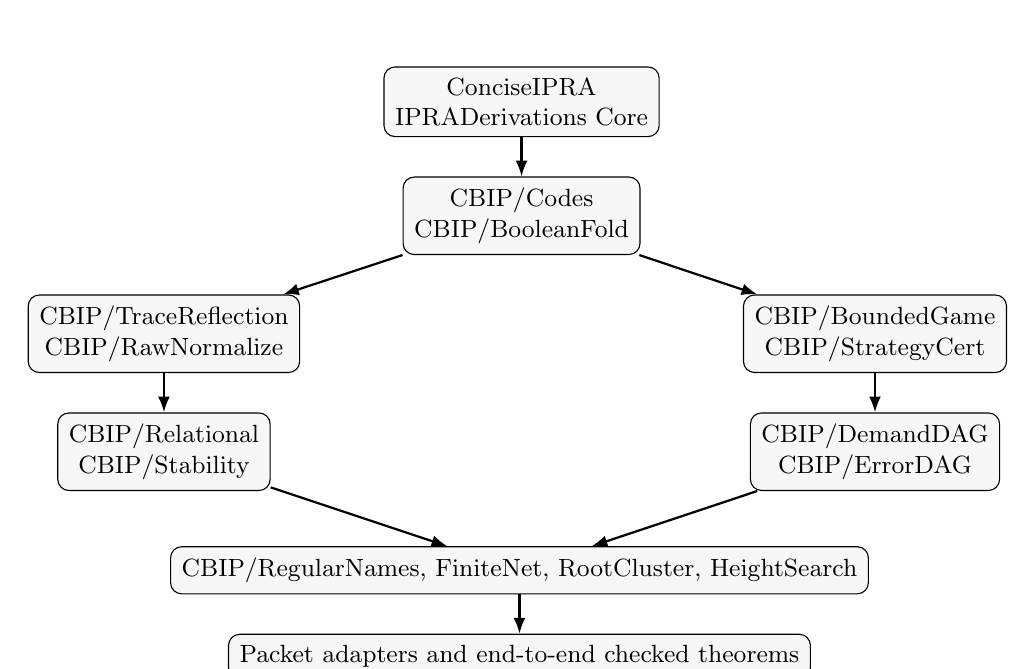
\begin{tikzpicture}[
 node distance=5mm and 13mm,
 box/.style={draw,rounded corners,align=center,fill=codegray,inner sep=4pt,font=\small},
 arr/.style={-{Latex[length=2mm]},thick}
]
\node[box] (up) {ConciseIPRA\\IPRADerivations Core};
\node[box,below=of up] (codes) {CBIP/Codes\\CBIP/BooleanFold};
\node[box,below left=of codes] (trace) {CBIP/TraceReflection\\CBIP/RawNormalize};
\node[box,below right=of codes] (game) {CBIP/BoundedGame\\CBIP/StrategyCert};
\node[box,below=of trace] (rel) {CBIP/Relational\\CBIP/Stability};
\node[box,below=of game] (err) {CBIP/DemandDAG\\CBIP/ErrorDAG};
\node[box,below=12mm of $(rel)!0.5!(err)$] (obj) {CBIP/RegularNames, FiniteNet, RootCluster, HeightSearch};
\node[box,below=of obj] (apps) {Packet adapters and end-to-end checked theorems};
\draw[arr] (up)--(codes);
\draw[arr] (codes)--(trace);
\draw[arr] (codes)--(game);
\draw[arr] (trace)--(rel);
\draw[arr] (game)--(err);
\draw[arr] (rel)--(obj);
\draw[arr] (err)--(obj);
\draw[arr] (obj)--(apps);
\end{tikzpicture}
\end{center}

\subsection{Dependency-ordered completion plan}

\begin{enumerate}
\item Compile the no-placeholder normalized reflection kernel.
\item Complete \code{normalizeRaw} using \code{inst}, \code{run_zero}, \code{run_succ}, and equality transport.
\item Reuse or promote checked Boolean, pairing, and search modules into a stable public API.
\item Prove \code{allBelow}/\code{anyBelow} elimination and introduction lemmas.
\item Complete one fixed \(\forall\exists\forall\) strategy certificate end to end.
\item Implement rectangular viability and least-viable replay.
\item Implement stable quotient/diameter erasure using the already compiled observable-glue pattern.
\item Add regular-name addition, product, and guarded reciprocal.
\item Add error-DAG and finite-net argmin.
\item Port one substantial packet end to end; good candidates are a separated rotation theorem, a finite-law probability estimate, or a root-cluster symmetric identity.
\item Only after correctness, optimize proof size or target the compressed native calculi.
\end{enumerate}

\subsection{Audits for every exported theorem}

A completed module should pass all of the following:

\begin{itemize}
\item clean \code{lake build};
\item source scan for \code{sorry}, \code{admit}, and newly introduced axioms;
\item \code{#print axioms} on each public theorem;
\item theorem type is visibly \code{Prf PRAAx} before any native export;
\item exact finite regression tests for the associated evaluator/checker;
\item a ledger entry naming every unresolved external producer.
\end{itemize}

\section{Worked examples}

\subsection{A bounded \texorpdfstring{\(\forall\exists\forall\)}{forall-exists-forall} contract}

Consider the finite statement
\[
  \forall q<Q\;\exists z<2Q+1\;\forall e<q+1\quad z+e\geq q.
\]
For each \(q<Q\), choose \(z=q\).  Since \(q<2Q+1\) and \(e\geq0\), every local test passes.  The positive strategy certificate stores the table \(z(q)=q\); the checker verifies the bounds and each inequality by finite loops.

The same compiled game also has informative failure behavior when the witness bound is changed to \(z<q\) and the test becomes \(z\geq q\).  It returns the least failing challenge \(q>0\), and for every candidate \(z<q\) it returns the test \(e=0\) witnessing failure.  This small example exercises dependent bounds, adversarial checks, success strategies, and counterstrategies without any unbounded reasoning.

\subsection{Relational square-root approximation}

For \(a=2\), at precision level \(n\) enumerate dyadic candidates
\[
  C_n=\left\{\frac{j}{2^n}:0\leq j\leq2^{n+2},\quad
  \left|\left(\frac{j}{2^n}\right)^2-2\right|\leq 4\cdot2^{-n}\right\}.
\]
All tests become integer inequalities after multiplying by \(2^{2n}\).  Let candidates at adjacent levels be compatible when
\[
  |q-r|\leq 2^{1-n}.
\]

A finite-horizon consumer asks only for levels up to \(h\).  The evidence machine's state contains the current level and the last candidate; local validity checks membership in \(C_n\) and compatibility.  Backward viability marks candidates that can reach level \(h\); forward execution chooses the least viable chain.

Nonemptiness can be proved by a bounded least-crossing search.  Let \(j_n\) be the least integer satisfying \(j_n^2\geq2^{2n+1}\), and put \(q_n=(j_n-1)/2^n\).  Then
\[
  q_n^2<2\leq(q_n+2^{-n})^2,
\]
so
\[
  0<2-q_n^2\leq2q_n2^{-n}+2^{-2n}\leq4\cdot2^{-n}.
\]
A direct comparison of adjacent crossing integers gives the compatibility bound.  Thus every finite horizon is viable.

A consumer that asks only for a residual bound or for a symmetric expression can use the chain and erase its internal choices.  The framework does not infer that the least chains for all \(h\) are prefixes of one another.  A coherent square-root name is obtained separately from uniqueness/monotonicity, not from viability alone.

\subsection{Guarded reciprocal with an explicit margin}

Suppose samples \(a(n)\) satisfy \eqref{eq:regular}, and the input includes a rational \(\alpha>0\) with \(|x|\geq\alpha\).  To compute an inverse sample of precision \(k\), choose \(n\) so that
\[
  2^{-n+1}\leq\alpha/2,
  \qquad
  \frac{8\cdot2^{-n}}{\alpha^2}\leq2^{-k-2}.
\]
Both inequalities are decided by bounded doubling searches.  Set \(b(k)=1/a(n)\) using the totalized rational reciprocal.

Regularity gives \(|a(n)|\geq\alpha/2\), so the numerator is nonzero.  For later requested samples \(a(m)\),
\[
 |b(k)-1/a(m)|\leq \frac{4|a(n)-a(m)|}{\alpha^2}
 \leq \frac{8\cdot2^{-n}}{\alpha^2}\leq2^{-k-2}.
\]
The CBIP state records the selected \(n\), the cross-multiplied guard, and the error inequality.  The terminal observer returns the rational inverse sample; no semantic real or partial function occurs in the object formula.

\subsection{Finite-net approximate minimization}

On \([0,2]\), let \(R(y)=|y^2-2|\).  For \(y,z\in[0,2]\),
\[
  |R(y)-R(z)|\leq|y^2-z^2|=|y-z||y+z|\leq4|y-z|.
\]
Use the dyadic grid \(G_n=\{j/2^n:0\leq j\leq2^{n+1}\}\).  Evaluate the residual exactly and choose the least grid minimizer by bounded search.  A least-crossing argument supplies a grid point within \(2^{-n}\) of \(\sqrt2\) in the explanatory metatheory, while internally the same integer crossing proves directly that its residual is at most \(4\cdot2^{-n}\).  The selected minimizer has no larger residual.

This proof uses a finite cover, a Lipschitz estimate, exact rational evaluation, and an argmin invariant.  It does not use an abstract extreme-value theorem.  If a coherent positive root name is desired, monotonicity and a separated positive interval turn residual bounds into distance bounds, yielding nested isolating intervals.

\subsection{Height-bounded enumeration}

For the equation \(x^2+y^2=5\), suppose the producer supplies \(\max(|x|,|y|)\leq3\).  Enumerate the finite box \([-3,3]^2\), test the equation, and canonically sort successful pairs.  The list is
\[
  (\pm1,\pm2),\qquad(\pm2,\pm1).
\]
The checker proves:
\begin{enumerate}
\item every listed pair satisfies the equation;
\item the list has no duplicates under the chosen encoding;
\item any solution obeying the supplied height bound occurs in the enumerated box and therefore in the list.
\end{enumerate}
The same generic program works after replacing the elementary bound by a Runge, Baker, descent, or other verified height certificate.  The generic program does not prove that certificate.

\subsection{A uniform metastability selector without a uniform rate}

For a simulated machine \(e\), use the sequence \(x_e(n)\in\{0,1\}\) from \Cref{sec:barriers}.  Given a finite challenge \(g\), simulate \(e\) for \(g(0)\) steps.  If no halt occurs, return the stable window starting at zero.  If the first halt occurs at \(t\leq g(0)\), return the window starting at \(t\).  The selector is a bounded program, and its certificate checks every term in the chosen interval.

This is a useful regression example because it formally prevents an invalid API design.  A type called \code{Metastable} must expose a challenged window, not a tail modulus.  Any coercion from the former to the latter would contradict the computability argument of \Cref{sec:barriers}.

\section{Theorem ledger, validation status, and further questions}

\subsection{Main claims}

\begin{longtable}{@{}p{0.42\textwidth}p{0.50\textwidth}@{}}
\toprule
Claim & Status in this artifact \\
\midrule
\endfirsthead
\toprule
Claim & Status in this artifact \\
\midrule
\endhead
Finitary presentation interface & Fully developed definition and examples \\
Two-sided bounded strategy compilation & Complete human proof; exact Python implementation for a finite syntax; Lean blueprint \\
Finite challenge decomposition & Complete human corollary and executable examples \\
Normalized trace reflection & Complete human proof; no-placeholder Lean candidate; not compiled here \\
Fixed-program CBIP normalization & Detailed structural proof schema; compiler implementation remains a Lean engineering task \\
Adaptive finite use of global hypotheses & Complete human invariant argument \\
Finite-use relational composition & Complete human proof; exact Python implementation/tests \\
Stable quotient and diameter witness erasure & Complete human proof; upstream packet supplies compiled generic logical glue, not rebuilt here \\
Regular-name arithmetic and guarded inverse & Complete quantitative arguments; object rational library/adapters remain to be implemented \\
Error-DAG soundness & Complete human proof; exact rational implementation/tests \\
Rank-to-metastability & Complete human proof and finite tests \\
Finite-net minimization and height/list conversion & Complete human proofs and exact reference implementations \\
Barrier reductions & Explicit halting-encoded arguments supplied \\
Full CBIP-to-\code{Prf PRAAx} metacompiler & Not implemented or kernel checked in this artifact \\
General deep producer theorems & Not claimed \\
\bottomrule
\end{longtable}

\subsection{Artifact validation}

The archive contains:
\begin{itemize}
\item LaTeX sources and the compiled report;
\item exact Python algorithms for bounded search, finite games, deterministic traces, relational viability, error DAGs, finite argmin, and bounded enumeration;
\item executed unit-test output;
\item a source-oriented no-placeholder normalized reflection candidate;
\item a larger Lean blueprint with explicit unfinished milestones;
\item machine-readable theorem and difficulty ledgers;
\item a source audit with the inspected repository hashes;
\item PDF preflight, render inspection, and checksum records.
\end{itemize}

Passing Python tests establishes behavior of finite reference algorithms on tested instances.  It does not establish their universal theorems in iPRA.  The Lean candidate has not been elaborated in this runtime.  Its no-placeholder status is therefore a stronger source claim than a file full of \code{sorry}, but weaker than a successful kernel build.

\subsection{Recommended end-to-end pilot}

The next decisive milestone is not another broad packet.  It is one substantial theorem carried through every layer:
\begin{enumerate}
\item explicit finite interface and producer assumptions;
\item concrete \code{PR} symbols;
\item normalized trace obligations;
\item completed \code{Prf PRAAx} proof;
\item native export;
\item axiom audit;
\item independent exact tests.
\end{enumerate}

A good pilot should exercise relational or guarded structure while avoiding an unresolved producer.  Candidates include a separated-real Euler--Rodrigues theorem with projective axis output, a finite-law Berry--Esseen core with a supplied moment budget, or a symmetric polynomial identity from a certified real-root clustering.

\subsection{Further research questions}

\begin{enumerate}
\item Can the raw-to-normalized trace elaborator be completed using only the existing checked instantiation, induction, congruence, and recursion APIs, with no new logical lemmas?
\item What is the smallest stable public API for Booleans, pairs, lists, bounded folds, and table updates that avoids repeated encodings across packets?
\item Can a Lean metaprogram generate \code{PR} syntax and \code{Prf PRAAx} local proofs from a typed CBIP while keeping the generated theorem readable?
\item How compact can two-sided strategy certificates be made for deeply alternating bounded formulas without complicating the trusted checker?
\item For relational viability, when is recomputation smaller than a sparse external DAG certificate?
\item Can demand and error scheduling be proof-producing, so an untrusted optimizer emits only a checkable budget certificate?
\item Which exact quotient representations cover the largest number of geometry and spectral packets: projective points, projectors, Pluecker coordinates, or finite chart families?
\item Can root-cluster refinement be formalized first for real Sturm intervals and then lifted to robust complex disks?
\item Which packet difficulties become Type I after importing the current checked order, search, gcd, division, and matrix libraries?
\item Can the barrier examples be turned into a formal linter that warns when a requested API would imply an exact sign, rate, cutoff, or infinite selector?
\item What proof-term and checker-size savings result from ordinary \code{PRAAx}, the native scalar core, and specialized certificate checkers?
\item Can repository-wide metadata automatically distinguish human proof, executable evidence, checked host theorem, object derivation, native export, and unresolved producer?
\end{enumerate}

\appendix
\section{Auditable normal forms for theorem statements}

\subsection{Deterministic finite construction}

A deterministic theorem should be presented as
\[
  \forall x\quad \Good(x)=1\longrightarrow
  \Post(x,F(x))=1,
\]
where \(F\), \(\Good\), and \(\Post\) are fixed primitive-recursive symbols or finite-observation predicates.  The artifact names the trace, invariant, fuel, and local derivations.

\subsection{Precision-indexed construction}

A represented theorem should be presented as
\[
  \forall p\quad H(p)\longrightarrow
  \forall k\quad \Obs(p,k,A(p,k))=1.
\]
The proof keeps \(p,k\) free, computes a finite query plan, proves the observation, and only then universally introduces \(k\).  The interface lists every modulus, magnitude bound, and guard consumed.

\subsection{Relational finite-use theorem}

A multivalued producer should expose
\[
  \forall x,h\quad \mathsf{Evidence}(x,h)=1\longrightarrow
  \Viable(x,h,\mathsf{start}(x))=1.
\]
A consumer theorem concludes a successful finite transcript, a quotient-invariant observation, or a diameter-stable output.  It must not silently replace finite viability by one infinite coherent selector.

\subsection{Alternating bounded contract}

A finite challenge theorem should expose both sides:
\[
 \CertCheck_A(x,1,c)=1\to A(x),\qquad
 \CertCheck_A(x,0,c)=1\to\neg A(x).
\]
The canonical evaluator produces one of the two certificates.  This makes failed finite stages auditable and separates logical failure from a missing external producer.

\subsection{Conditional certificate theorem}

For an external certificate \(c\), state
\[
  \forall x,c\quad \CertCheck(x,c)=1\longrightarrow
  \Phi(x,\mathsf{out}(c)).
\]
Record separately whether a producer is known for all admissible \(x\), for a special family, or only experimentally.

\subsection{Exact branch under a gap}

An exact selector should have the guarded form
\[
  \mathsf{Gap}(x,m)=1\longrightarrow
  \mathsf{ExactBranch}(x,\mathsf{select}(x,m))=1.
\]
Without a gap, use overlapping branches, a finite relation, a cluster, a projective class, or a stable observation.

\subsection{Height and complete-list theorem}

A Diophantine enumeration theorem should name the effective producer:
\[
  \mathsf{CurveHyp}(x)\longrightarrow
  \forall z\bigl(P(x,z)=1\to h(z)\leq B(x)\bigr),
\]
with concrete primitive-recursive \(B\), or else accept a supplied height certificate.  Only after this premise is available does the generic bounded enumerator yield a complete list.

\section{Notation and implementation conventions}

\begin{center}
\begin{tabularx}{\textwidth}{@{}lX@{}}
\toprule
Notation & Meaning \\
\midrule
\code{PR} & fixed primitive-recursive definition, never an unclocked universal evaluator \\
\(u,x,p\) & paired numerical input, parameter, or certificate codes \\
\(k\) & requested output precision \\
\(h,r\) & finite interaction horizon or remaining resource \\
\(s\) & encoded machine/consumer state \\
\(\Viable(x,r,s)\) & backward Boolean saying a successful finite continuation exists \\
\(\Local(x,r,s,a)\) & local admissibility of answer \(a\) \\
\(E\) & observational equivalence, not necessarily literal equality \\
\(\delta\) & output diameter or error bound \\
\(\Prf\ \PRAAx\ \Gamma\ \varphi\) & object-level derivability in ordinary iPRA \\
\bottomrule
\end{tabularx}
\end{center}

All finite sequences and graphs may use any standard primitive-recursive coding with explicit bounds.  Implementations should nonetheless share one canonical repository encoding to avoid repeated conversion theorems.  Rational inequalities are reduced to signed-integer cross products with positive denominators.  Every order decision is therefore an exact decision on finite codes, not an order decision on an arbitrary represented real.


\begin{thebibliography}{99}
\bibitem{proveit-readme}
V.~Reshetnikov, \emph{ProveIt: Primitive Recursive Arithmetic README}, repository snapshot \texttt{210616e660a7ab5f0d706761c12bba673174cec9}, 2026.

\bibitem{concise-ipra}
V.~Reshetnikov, \emph{ConciseIPRA: checked mutually bi-interpretable presentations of iPRA}, ProveIt repository, 2026.

\bibitem{ipra-derivations}
V.~Reshetnikov, \emph{IPRADerivations: kernel-checked object-language derivations}, ProveIt repository, 2026.

\bibitem{finite-use}
V.~Reshetnikov and collaborators, \emph{Demand-Driven Relational Certificates for Mathematics in iPRA}, ProveIt research packet, 2026.

\bibitem{contract-dag}
V.~Reshetnikov and collaborators, \emph{Certified Finitary Presentations and a Contract-DAG Compiler}, ProveIt research packet, 2026.

\bibitem{finitary-compiler}
V.~Reshetnikov and collaborators, \emph{Finitary Interfaces and Proof-Producing Compilation for iPRA}, ProveIt research packet, 2026.

\bibitem{bishop}
E.~Bishop and D.~Bridges, \emph{Constructive Analysis}, Springer, 1985.

\bibitem{bridges-richman}
D.~Bridges and F.~Richman, \emph{Varieties of Constructive Mathematics}, Cambridge University Press, 1987.

\bibitem{troelstra}
A.~S.~Troelstra and D.~van Dalen, \emph{Constructivism in Mathematics}, North-Holland, 1988.

\bibitem{kleene}
S.~C.~Kleene, \emph{Introduction to Metamathematics}, North-Holland, 1952.

\bibitem{kohlenbach}
U.~Kohlenbach, \emph{Applied Proof Theory: Proof Interpretations and Their Use in Mathematics}, Springer, 2008.
\end{thebibliography}

\end{document}
